\documentclass[tikz, border=10mm]{standalone}
\usepackage{amsmath, amssymb}
\usetikzlibrary{arrows.meta, bending, shapes.geometric, calc}

\begin{document}
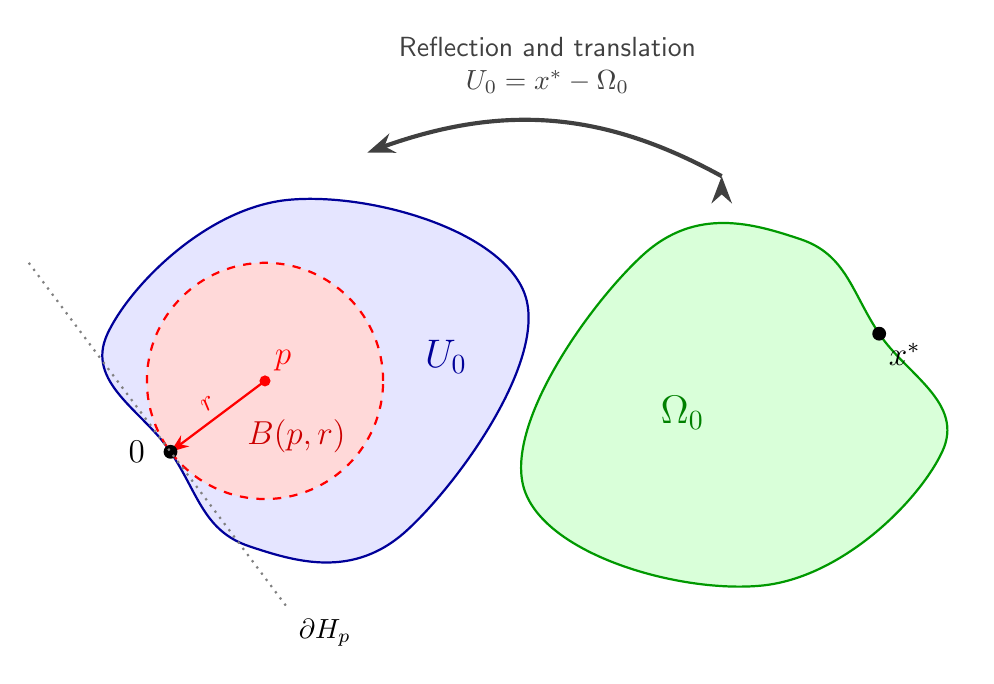
\begin{tikzpicture}[>=Stealth, font=\sffamily]

    % 1. Współrzędne kluczowych punktów
    \coordinate (O) at (0,0);           % Początek układu współrzędnych (0)
    \coordinate (xstar) at (9, 1.5);    % Punkt x^* leżący na brzegu \Omega_0
    
    % Środek kuli wpisanej B(p, r) dobrany tak, by r było mniejsze.
    % Promień to odległość od (1.2, 0.9) do (0,0), czyli sqrt(1.2^2 + 0.9^2) = 1.5
    \coordinate (p) at (1.2, 0.9);      
    \def\r{1.5}

    % Definicja krzywej ograniczającej zbiór U_0.
    % Odpowiednio ukształtowana, żeby mała kula była głęboko wewnątrz.
    \def\Upath{plot[smooth cycle, tension=0.7] coordinates {
        (0,0) 
        (-0.8, 1.5) 
        (1.5, 3.2) 
        (4.5, 2.0) 
        (3.0, -1.0) 
        (1.0, -1.2)
    }}

    % 2. RYSOWANIE ZBIORU \Omega_0
    % Matematycznie: U_0 = x^* - \Omega_0, czyli \Omega_0 = x^* - U_0.
    % Transformacja to nałożenie ujemnej skali (odbicie) i przesunięcia o x^*.
    \begin{scope}[shift={(xstar)}, xscale=-1, yscale=-1]
        \draw[fill=green!15, draw=green!60!black, thick] \Upath;
        \node[text=green!50!black] at (2.5, 1.0) {\Large $\Omega_0$};
        
        % Punkt x^* w lokalnym układzie
        \fill[black] (0,0) circle (2.5pt);
        \node[below right, font=\large] at (0,0) {$x^*$};
    \end{scope}

    % 3. RYSOWANIE ZBIORU U_0
    \draw[fill=blue!10, draw=blue!60!black, thick] \Upath;
    
    % Podpis dla U_0 umieszczony po prawej stronie (poza kulką)
    \node[text=blue!60!black, font=\Large] at (3.5, 1.2) {$U_0$};

    % 4. RYSOWANIE KULI B(p, r)
    \draw[fill=red!15, draw=red, thick, dashed] (p) circle (\r);
    
    % Wyraźny podpis dla kuli
    \node[text=red!80!black, font=\large] at (1.6, 0.2) {$B(p, r)$};
    
    % Punkt środka p i strzałka promienia
    \fill[red] (p) circle (2pt) node[above right, text=red, font=\large] {$p$};
    \draw[->, red, thick] (p) -- node[above, sloped] {$r$} (O);

    % Punkt 0 (początek układu współrzędnych)
    \fill[black] (O) circle (2.5pt) node[left=2mm, font=\large] {$0$};

    % 5. PÓŁOKRĄGŁA STRZAŁKA TRANSFORMACJI
    \draw[->, line width=1.5pt, darkgray] 
        (7, 3.5) edge[bend right=25] 
        node[above, align=center, yshift=2mm] {Reflection and translation \\ $U_0 = x^* - \Omega_0$} (2.5, 3.8);

    % 6. PÓŁPRZESTRZEŃ H_p (Zgodnie z dowodem)
    % Jest to linia prostopadła do wektora p przechodząca przez 0
    \draw[thick, gray, dotted] (-1.8, 2.4) -- (1.5, -2.0) node[below right, text=black] {$\partial H_p$};

\end{tikzpicture}
\end{document}